% !TEX root = ./Basilisk-houghCircles-20190213.tex

\section{Test Description and Success Criteria}
In order to test the proper function of this module, two test images are provided.
The algorithm needs to find all the circles in the images within 1 pixel of relative error.

\section{Test Parameters}

\begin{table}[htbp]
	\caption{Error tolerance for each test.}
	\label{tab:errortol}
	\centering \fontsize{10}{10}\selectfont
	\begin{tabular}{ c | c | c  } % Column formatting, 
		\hline\hline
		\textbf{Test image}  & Expected Circles & \textbf{Tolerated Error}  \\  \hline
		mars    & 1 &1 px	   \\ 
		moons        & 6 &1 px   \\ 
		\hline\hline
	\end{tabular}
\end{table}


\section{Test Results}
The following table shows the results of the unit test described above.

\begin{table}[H]
	\caption{Test results}
	\label{tab:results}
	\centering \fontsize{10}{10}\selectfont
	\begin{tabular}{c | c  } % Column formatting, 
		\hline\hline
		\textbf{Check} 						  		&\textbf{Pass/Fail} \\ 
		\hline
	   mars   			& PASS \\ 
	   moons   			& PASS  \\
	   \hline\hline
	\end{tabular}
\end{table}

The test does not generate the result image unless called explicitly from python in order to not add images to the repository.

\begin{figure}[h!]
\centering
  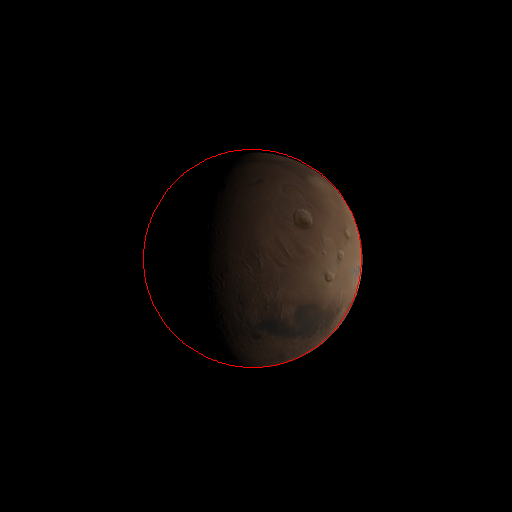
\includegraphics[width = 0.5\linewidth]{../_UnitTest/result_mars.png}
  \caption{Mars Circles}
  \label{fig:mars}
\end{figure}

\begin{figure}[h!]
\centering
  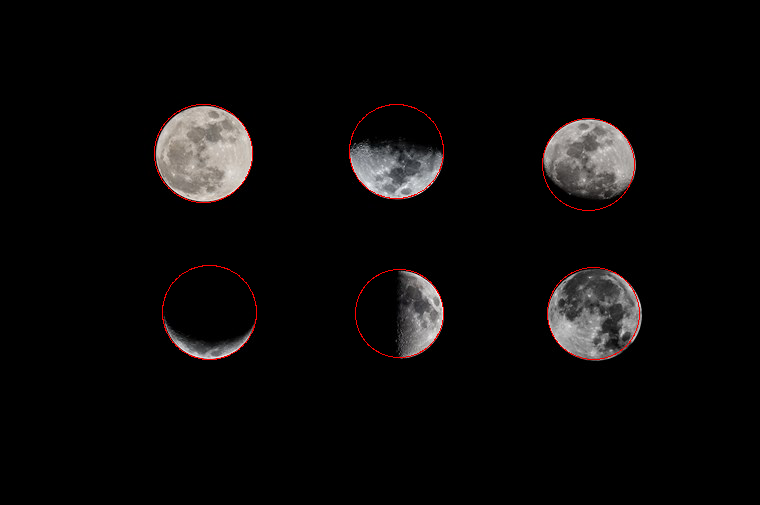
\includegraphics[width = 0.5\linewidth]{../_UnitTest/result_moons.png}
  \caption{Moon crescents circles}
  \label{fig:moons}
\end{figure}

